\documentclass[]{article}
\usepackage{polski} 
\usepackage[utf8]{inputenc}

\usepackage{listings}
\usepackage{xcolor}
\lstdefinestyle{sharpc}{
	language=[Sharp]C,
	basicstyle=\footnotesize\ttfamily,
	numbers=left,
	numberstyle=\tiny,
	numbersep=5pt,
	tabsize=2,
	extendedchars=true,
	breaklines=true,
	frame=b,
	stringstyle=\color{blue}\ttfamily,
	showspaces=false,
	showtabs=false,
	xleftmargin=17pt,
	framexleftmargin=17pt,
	framexrightmargin=5pt,
	framexbottommargin=4pt,
	commentstyle=\color{green},
	morecomment=[l]{//}, %use comment-line-style!
	morecomment=[s]{/*}{*/}, %for multiline comments
	showstringspaces=false,
	keywordstyle=\color{purple},
	identifierstyle=\color{blue},
	backgroundcolor=\color{white},
	morekeywords={
		abstract, event, new, struct,
		as, explicit, null, switch,
		base, extern, object, this,
		bool, false, operator, throw,
		break, finally, out, true,
		byte, fixed, override, try,
		case, float, params, typeof,
		catch, for, private, uint,
		char, foreach, protected, ulong,
		checked, goto, public, unchecked,
		class, if, readonly, unsafe,
		const, implicit, ref, ushort,
		continue, in, return, using,
		decimal, int, sbyte, virtual,
		default, interface, sealed, volatile,
		delegate, internal, short, void,
		do, is, sizeof, while,
		double, lock, stackalloc,
		else, long, static,
		enum, namespace, string
	}
}
\lstset{style=sharpc}

\usepackage{geometry}
\newgeometry{tmargin=3cm, bmargin=3cm, lmargin=3.5cm, rmargin=3.5cm}
\linespread{1.25}

\usepackage{graphicx}
\graphicspath{ {./figures/} }
\usepackage{float}
\usepackage{subfig}

\title{Aplikacja webowa z przydomkami klubów}
\author{Sebastian Tyda}

\begin{document}

\maketitle
\tableofcontents

\newpage
\section*{Wstęp}
Celem projektu było stworzenie aplikacji MVC w technologii .NET do przeglądania i modyfikowania przydomków klubów piłkarskich. 

\section{Modele danych}
W projekcie uwzględniono trzy podstawowe modele danych:
\begin{itemize}
	\item \textbf{Country}, reprezentujący kraj
	\item \textbf{Team}, reprezentujący drużynę piłkarską
	\item \textbf{Nickname}, reprezentujący przydomek klubu
\end{itemize}

\subsection{Country}
Istotą klasy $Country$ jest możliwość grupowania klubów piłkarskich po kraju z jakiego pochodzą.
\begin{lstlisting}
public class Country
{
	public int Id { get; set; }
	public string Name { get; set; }
	public IList<Team>? Teams { get; set; }
}
\end{lstlisting}
Parametr $Id$ jest unikalnym identyfikatorem każdego kraju, parametr $Name$ jest to nazwa kraju, np. $Italy$. Pole $Teams$ służy do wygodnego odpytania o wszystkie drużyny z danego kraju, bez potrzeby dodatkowych linijek kodu, wystarczy odwołanie do tej zmiennej.

\subsection{Team}
Zadaniem klasy $Team$ jest przechowywanie danych na temat każdego klubu.
\begin{lstlisting}
public class Team
{
	public int Id { get; set; }
	public string Name { get; set; }
	public int CountryId { get; set; }
	public Country? Country { get; set; }
	public IList<Nickname>? Nicknames { get; set; }
}
\end{lstlisting}
Parametr $Id$ jest unikalnym identyfikatorem każdego klubu, parametr $Name$ jest to nazwa klubu, np. $Juventus$. $CountryId$ to klucz obcy, realizujący relację one to many z modelem $Country$. Podobnie jak wcześniej istnieją tu pola pomocnicze do poruszania się po relacjach.

\subsection{Nickname}
Klasa $Nickname$ umożliwia przechowywanie informacji o przydomkach klubów piłkarskich.
\begin{lstlisting}
public class Nickname
{
	public int Id { get; set; }
	public string Name { get; set; }
	public int TeamId { get; set; }
	public Team? Team { get; set; }
}
\end{lstlisting}
Parametr $Id$ jest unikalnym identyfikatorem każdego klubu, parametr $Name$ jest to nazwa przydomku, np. $The Old Lady$. $TeamId$ to klucz obcy, realizujący relację one to many z modelem $Team$. Podobnie jak wcześniej istnieją tu pola pomocnicze do poruszania się po relacjach.

\section{Widoki}

\subsection{Strona główna} \label{landing-page}
Strona główna aplikacji umożliwia wybór kraju, z którego odwiedzający stronę chciałby zobaczyć przydomki.

\begin{figure}[H]
	\centering
	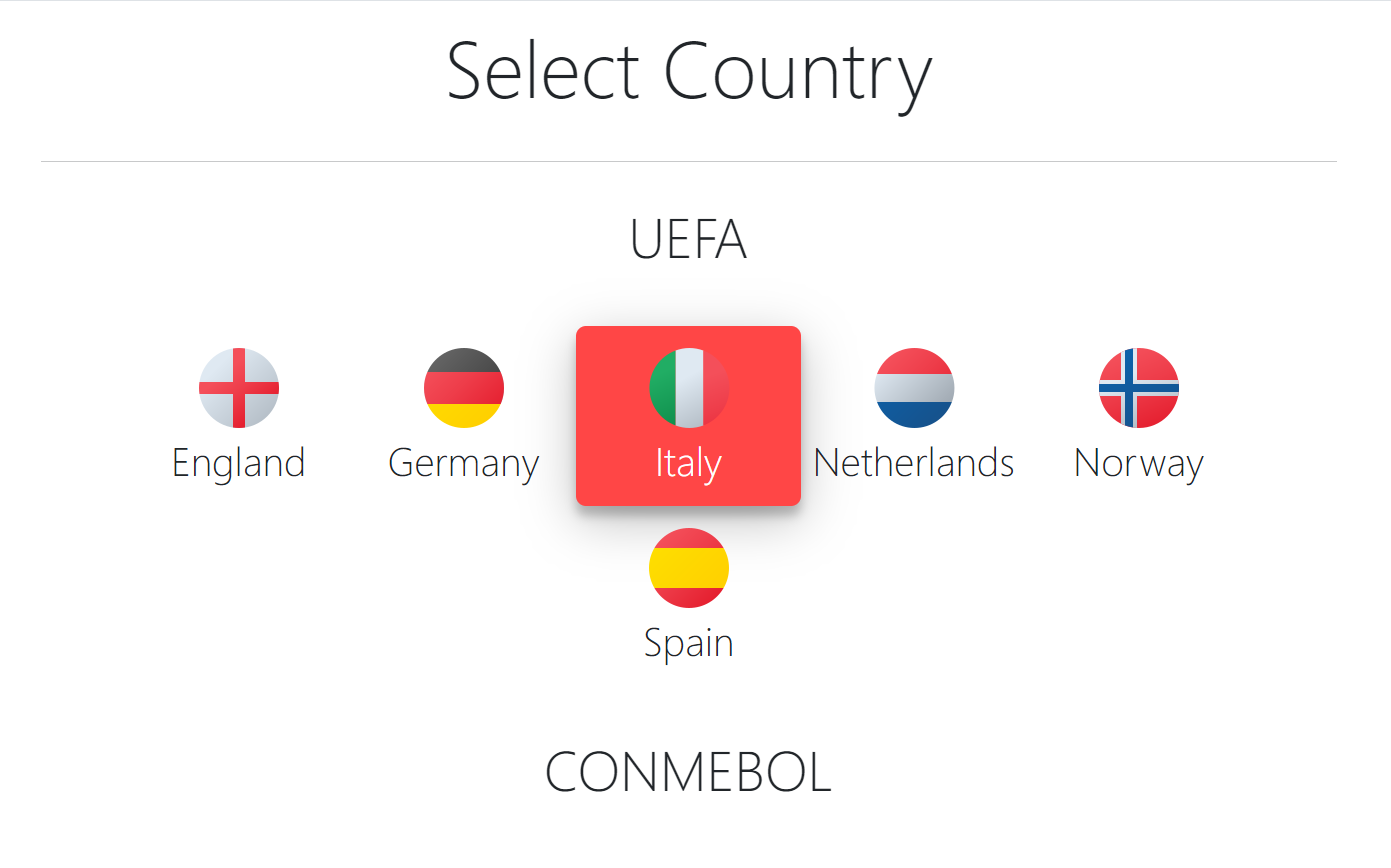
\includegraphics[scale=0.38]{landing-page}
	\caption{Strona główna - wybór kraju}
\end{figure}

\subsection{Lista przydomków} \label{nicknames-view}
Widok $CountryTeams$ umożliwia przeglądanie przydomków poszczególnych drużyn w formie prostej listy.

\begin{figure}[H]
	\centering
	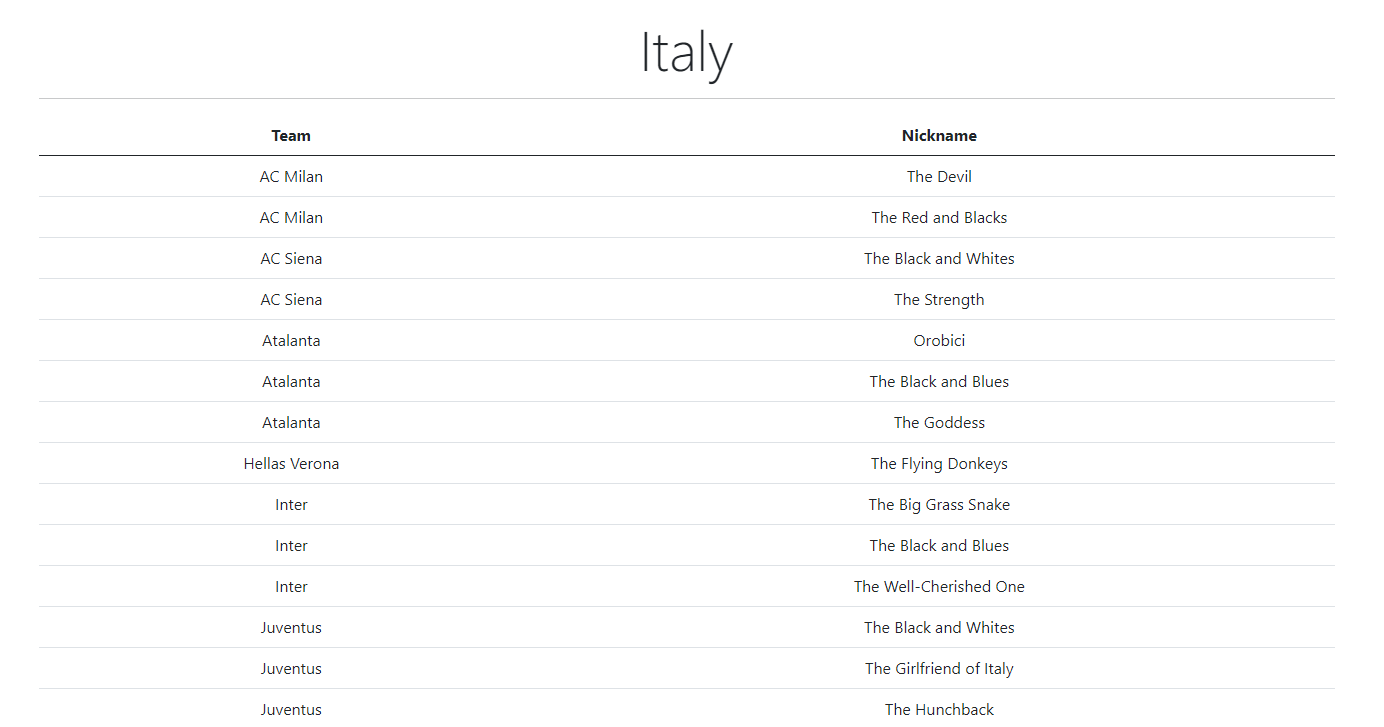
\includegraphics[scale=0.39]{nicknames-view}
	\caption{Lista przydomków}
\end{figure}

\subsection{Header} \label{header}
Nagłówek aplikacji różni się dla zalogowanych użytkowników. Zalogowany użytkownik jest adminem aplikacji. Z tego względu po zalogowaniu się w headerze pojawia się odnośnik do admin panelu.

\begin{figure}[H]%
	\centering
	\subfloat{{
\includegraphics[scale=0.8]{guest-header} }}%
	\qquad
	\subfloat{{
\includegraphics[scale=0.8]{admin-header} }}%
	\caption{Nagłówek gościa vs admina}%
\end{figure}

\subsection{Rejestracja oraz logowanie}
W prawym górnym rogu nagłówka są odnośniki do rejestracji i logowania. Na potrzeby projektu rejestrować może się każdy. Docelowo konta adminów byłyby tworzone odgórnie a rejestracja byłaby zablokowana.

\begin{figure}[H]%
	\centering
	\subfloat{{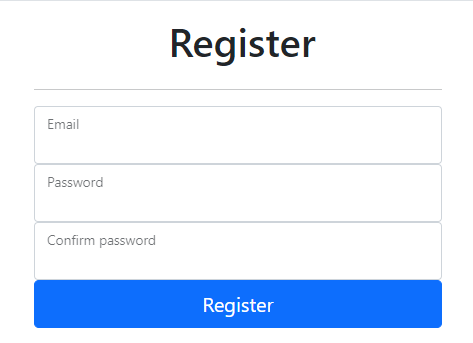
\includegraphics[width=5cm]{register} }}%
	\qquad
	\subfloat{{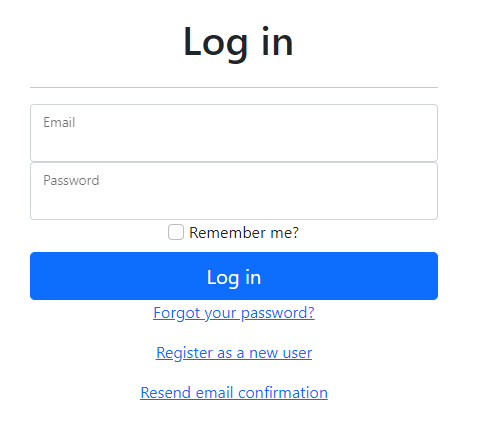
\includegraphics[width=5cm]{login} }}%
	\caption{Logowanie oraz rejestracja}%
\end{figure}

\subsection{Profil użytkownika}
Po zalogowaniu się w ramach profilu użytkownika mamy dostęp do prostych operacji typu zmiana hasła, maila czy usunięcie konta.

\begin{figure}[H]
	\centering
	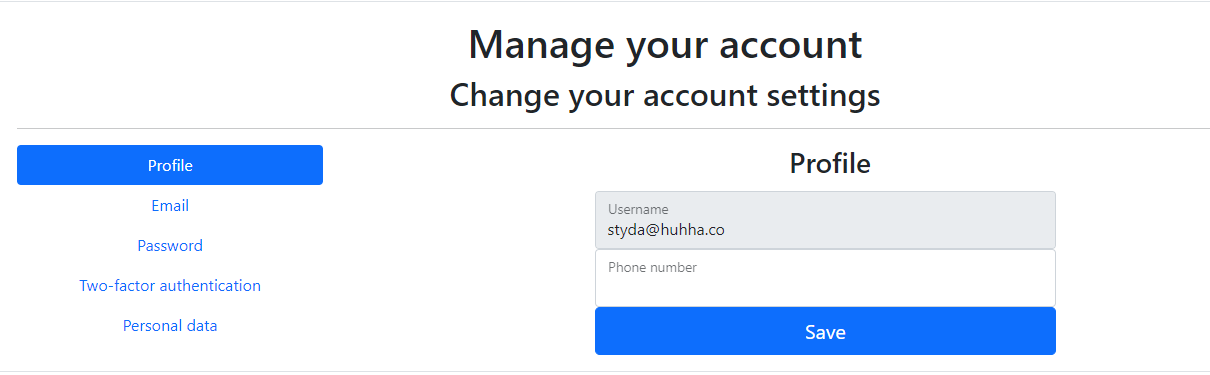
\includegraphics[scale=0.4]{profile}
	\caption{Profil}
\end{figure}

\subsection{Panel Admina}
Panel admina umożliwia crudowe zarządzanie bazą danych z poziomu aplikacji, a więc bez problemu możemy tutaj przeglądać, tworzyć, edytować i usuwać kraje, zespoły, jak i przydomki.

\begin{figure}[H]
	\centering
	
\includegraphics[scale=0.4]{admin-panel}
	\caption{Panel admina}
\end{figure}

\begin{figure}[H]
	\centering
	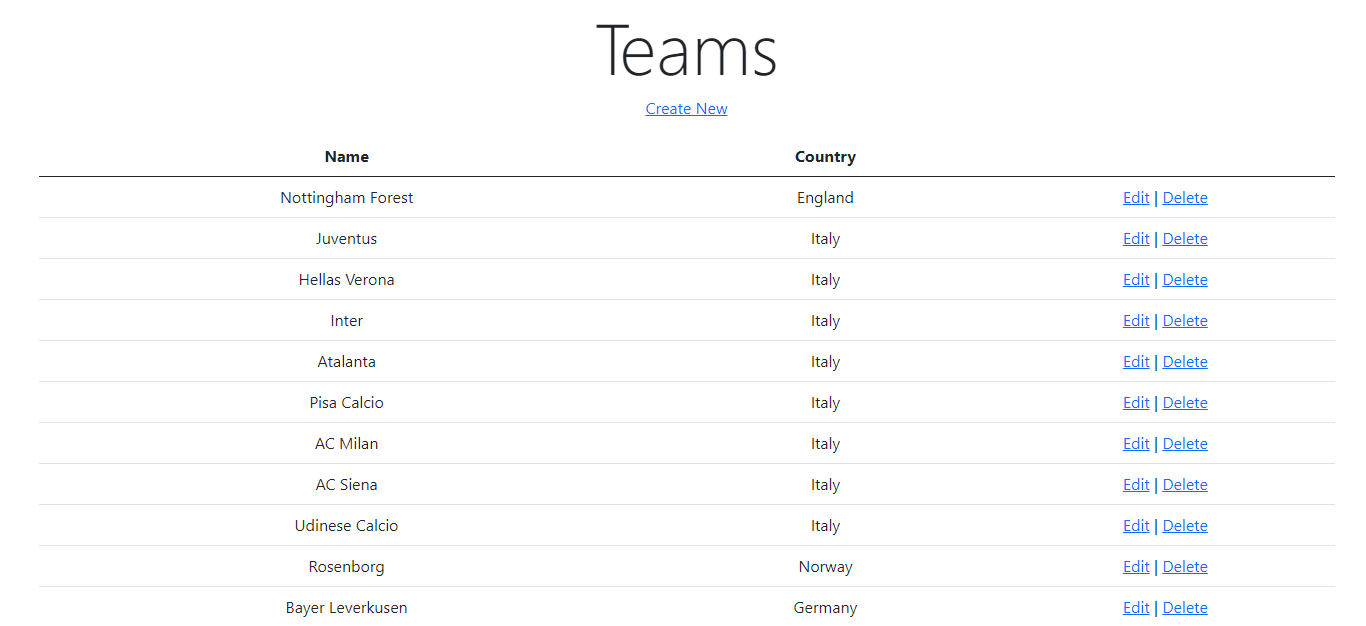
\includegraphics[scale=0.4]{admin-panel-teams}
	\caption{Panel admina - widok tabeli}
\end{figure}

\begin{figure}[H]%
	\centering
	\subfloat{{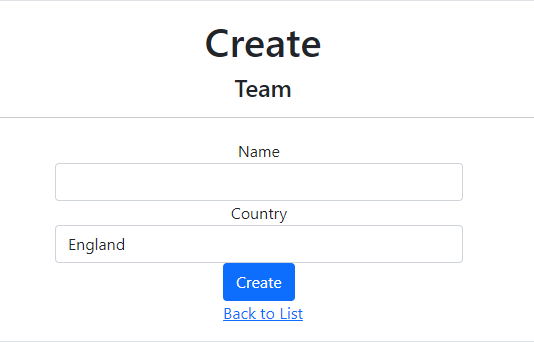
\includegraphics[scale=0.5]{team-create} }}%
	\qquad
	\subfloat{{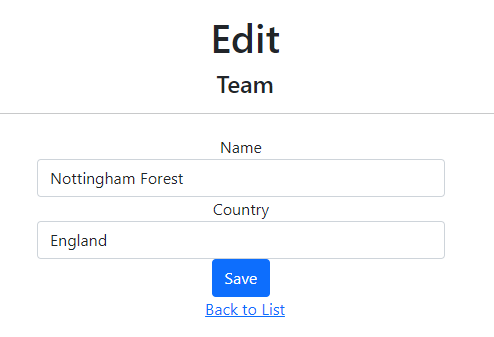
\includegraphics[scale=0.5]{team-edit} }}%
	\caption{Panel admina - dodawanie i edytowanie rekordu}%
\end{figure}

\begin{figure}[H]
	\centering
	
\includegraphics[scale=0.4]{team-delete}
	\caption{Panel admina - usuwanie rekordu}
\end{figure}

\end{document}
